本节对DEWP和TEMP两列分别使用Pandas进行了0-1归一化和Z-Score归一化处理,
并将结果使用matplotlib绘制饼图进行可视化处理.

\subsection{实现介绍}
0-1正规化, 将原始数据缩放到[0, 1]区间内:
\begin{equation}
    \frac{x-\min}{\max - \min}
\end{equation}
但是缺点是当新数据加入的时候, 可能导致最大和最小值发生变化, 从而需要重新计算.

z-Score, 将原始数据转换为标准正态分布:
\begin{equation}
    \frac{x-\mu}{\sigma}
\end{equation}
但是缺点是对原始数据的分布有要求, 即原始数据的分布必须是近似正态分布的.

\begin{lstlisting}[language=Python]
    min = df["DEWP"].min()
    max = df["DEWP"].max()

    # 0-1 normalization.
    def norm01(x, min, max): return (x - min) / (max - min)
    def norm01_col(col): return [norm01(col[i], min, max) for i in
                                 range(len(col))]

    df["DEWP"] = norm01_col(df["DEWP"])
    print(f"0-1 nomalized column 'DEWP'.")

    # Normalize column TEMP with Z-Score
    def norm_z(x, mean, std): return (x - mean) / std
    mean = df["TEMP"].mean()
    std = df["TEMP"].std()
    def norm_z_col(col): return [norm_z(col[i], mean, std) for i in
                                 range(len(col))]
    df["TEMP"] = norm_z_col(df["TEMP"])
    print(f"z-score normalized column 'TEMP'.") 
\end{lstlisting}

\subsection{处理结果}
\begin{lstlisting}
                         No  season  ...  DEWP   HUMI  PRES  TEMP ...
    Date
    2010-01-01 00:00:00   1       4  ...   -21   43.0  1021   -11 ...
    2010-01-01 01:00:00   2       4  ...   -21   47.0  1020   -12 ...
    2010-01-01 02:00:00   3       4  ...   -21   43.0  1019   -11 ...
    2010-01-01 03:00:00   4       4  ...   -21   55.0  1019   -14 ...
    2010-01-01 04:00:00   5       4  ...   -20    NaN  1018   -12 ...
    2010-01-01 05:00:00   6       4  ...   -19   47.0  1017   -10 ...
    2011-01-01 06:00:00   7       4  ...   -19   44.0  1017    -9 ...
    2010-01-01 07:00:00   8       4  ...   -19  440.0  1017    -9 ...
    2010-01-01 08:00:00   9       4  ...   -19   44.0  1017    -9 ...
    2010-01-01 09:00:00  10       4  ...   -20   37.0  1017    -8 ...

    ...
    0-1 nomalized column 'DEWP'.
    z-score normalized column 'TEMP'.
                         No  season  ...  DEWP   HUMI  PRES      TEMP ...
    Date
    2010-01-01 00:00:00   1       4  ...   0.0   43.0  1021 -0.271607 ...
    2010-01-01 01:00:00   2       4  ...   0.0   47.0  1020 -0.814822 ...
    2010-01-01 02:00:00   3       4  ...   0.0   43.0  1019 -0.271607 ...
    2010-01-01 03:00:00   4       4  ...   0.0   55.0  1019 -1.901251 ...
    2010-01-01 04:00:00   5       4  ...   0.5   51.0  1018 -0.814822 ...
    2010-01-01 05:00:00   6       4  ...   1.0   47.0  1017  0.271607 ...
    2010-01-01 06:00:00   7       4  ...   1.0   44.0  1017  0.814822 ...
    2010-01-01 07:00:00   8       4  ...   1.0  440.0  1017  0.814822 ...
    2010-01-01 08:00:00   9       4  ...   1.0   44.0  1017  0.814822 ...
    2010-01-01 09:00:00  10       4  ...   0.5   37.0  1017  1.358036 ...
\end{lstlisting}
可以看到DEWP中数据被0-1正规化, 而TEMP中数据被z-score正规化.

\subsection{可视化结果}
由于测试集的数据规模较小, 不能很好的体现正规化后的特征,
因此使用北京PM完整数据集对0-1正规化和z-score正规化的数据使用散点图进行展示如图.
\begin{figure}
    \centering
    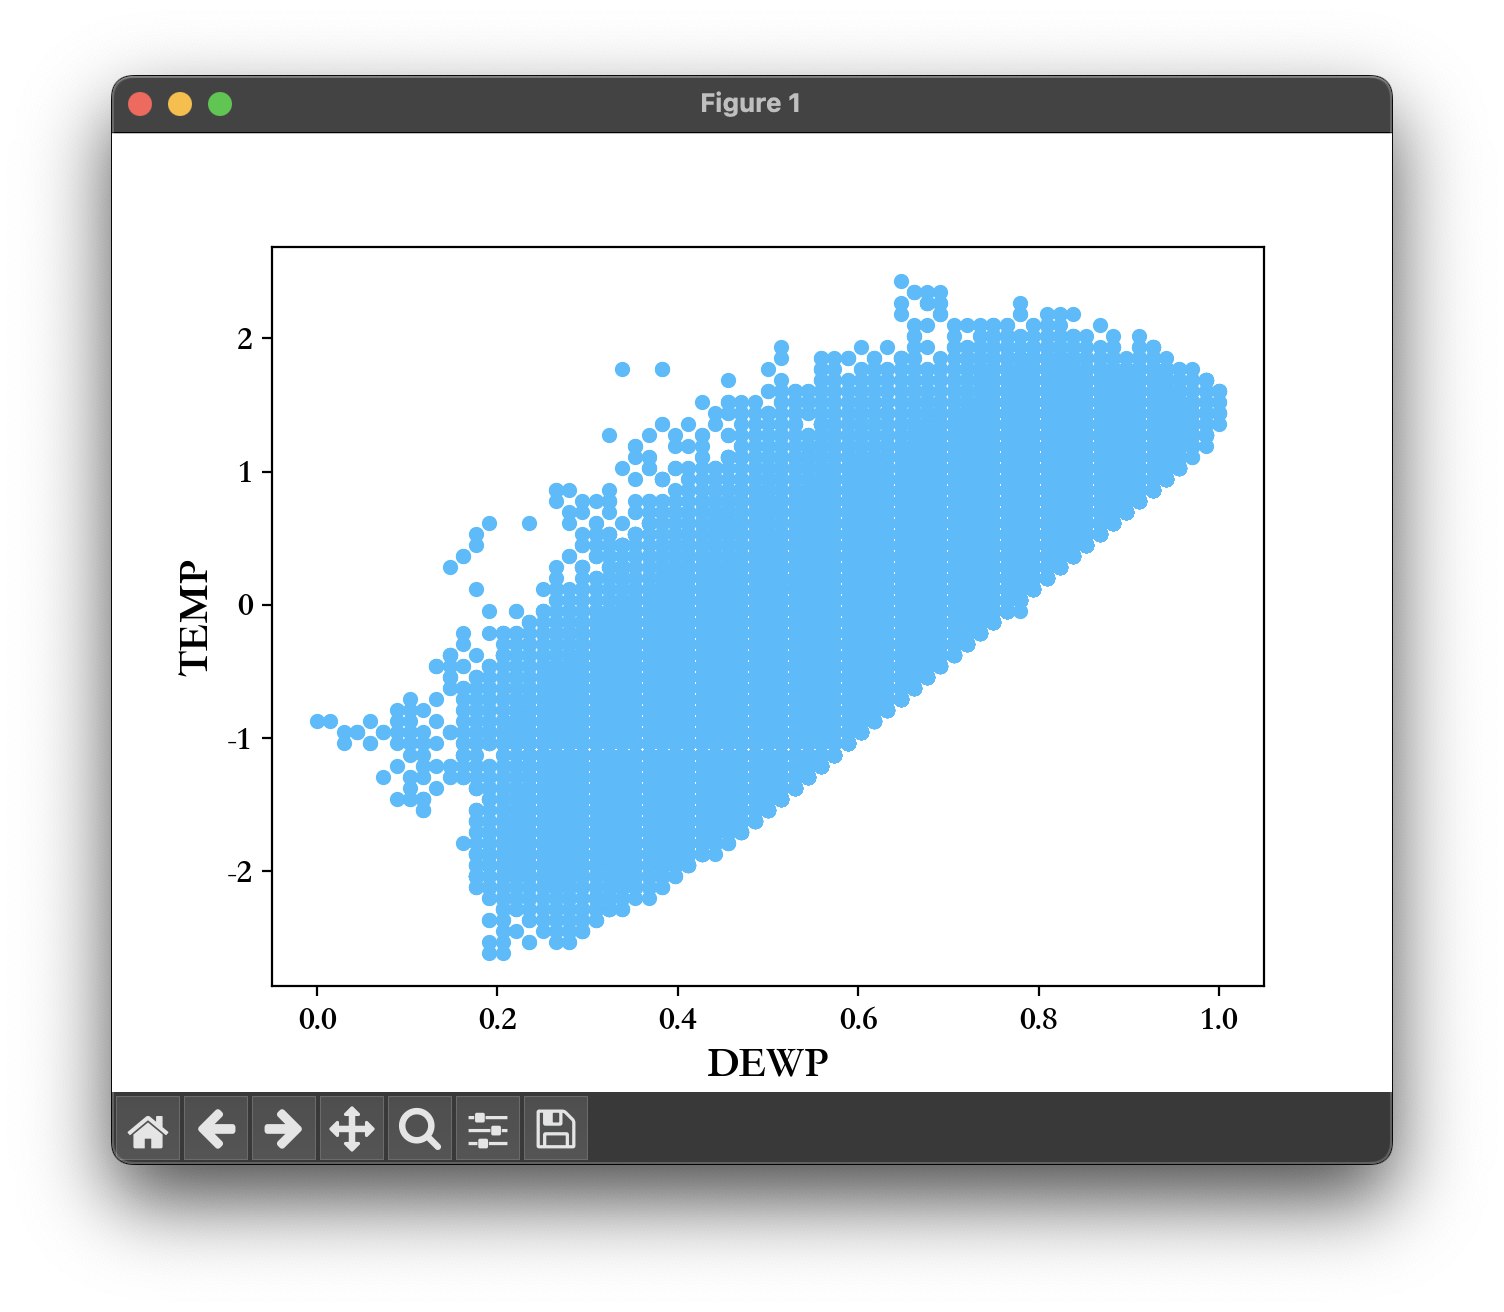
\includegraphics[width=0.8\textwidth]{figures/normalized-scatter.png}
    \label{fig:0-1正规化和z-score正规化散点图}
    \caption{0-1正规化和z-score正规化散点图}
\end{figure}